\documentclass[10pt]{beamer}
\usepackage[portuges]{babel}% Para adicionar a língua (PT)
\usepackage[utf8]{inputenc}
\usepackage{graphicx}
\usepackage{amsfonts}
\usepackage{xcolor}
\usepackage{amsmath}
\usepackage{amstext}
\usepackage{caption}
\usepackage{subcaption}

\usetheme{default}
\usecolortheme{dove}
\title[LFAOFR]{Espectroscopia $\beta$}
\institute{
Instituto Superior Técnico\\
\and
\inst{1} \tiny 78497 \; \inst{2} \tiny 78653 \; \inst{3} \tiny 78850 \; \inst{3} \tiny 78889 \\
}
\setbeamercovered{transparent}
\subtitle{\small \color{black} Mestrado em Engenharia Física Tecnológica\\
\footnotesize \color{black} LFAOFR}
\author{
Gonçalo Castro \inst{1}, António Costa \inst{2}, Miguel Gonçalves \inst{3}, Pedro Pereira \inst{4}
}

\date{\today}

\begin{document}

\begin{frame}
\titlepage
\end{frame}

%%%%%%%%%%%%%%%%%%%%%%%%%%%%%%%%%%%%%%%%%%%%%%%%%%%%

\begin{frame}
\frametitle{Decaimento $\beta$}

\begin{center}
$n \rightarrow p + e^{-} + \overline{\nu_{e}}$ 
\end{center}

\begin{figure}
\centering
\begin{subfigure}{.5\textwidth}
  \centering
  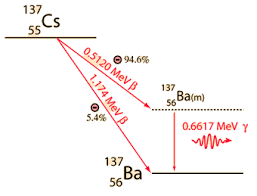
\includegraphics[scale=0.4]{cs.png}
\caption{Esquema Decaimento \ce{^{137}_{55}Cs}}
  \label{fig:sub1}
\end{subfigure}%
\begin{subfigure}{.5\textwidth}
  \centering
  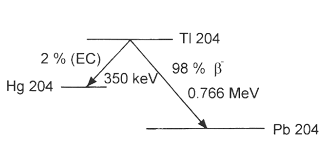
\includegraphics[scale=0.4]{tl.png}
\caption{Esquema Decaimento \ce{^{204}_{81}Tl}}
  \label{fig:sub2}
\end{subfigure}
\label{fig:test}
\end{figure}

\end{frame}

\begin{frame}
\frametitle{Electrões de conversão}

\begin{equation}
 p + e^{-} \rightarrow n + \nu_{e}
\end{equation}

\begin{figure}
  \centering
  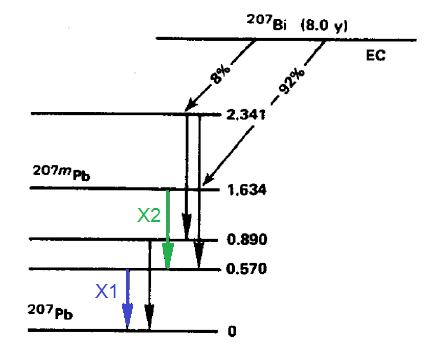
\includegraphics[scale=0.4]{bi.png}
\caption{Esquema Decaimento \ce{^{207}_{83}Bi}}
\label{fig:test}
\end{figure}


\begin{equation}
E_{e^-}=E_{X} -E_{L_{j}}
\label{Ee}
\end{equation}


\end{frame}

\begin{frame}
\frametitle{Montagem}
\framesubtitle{Detector semicondutor de barreira de superfície}

\begin{figure}
\centering
\begin{subfigure}{.5\textwidth}
  \centering
  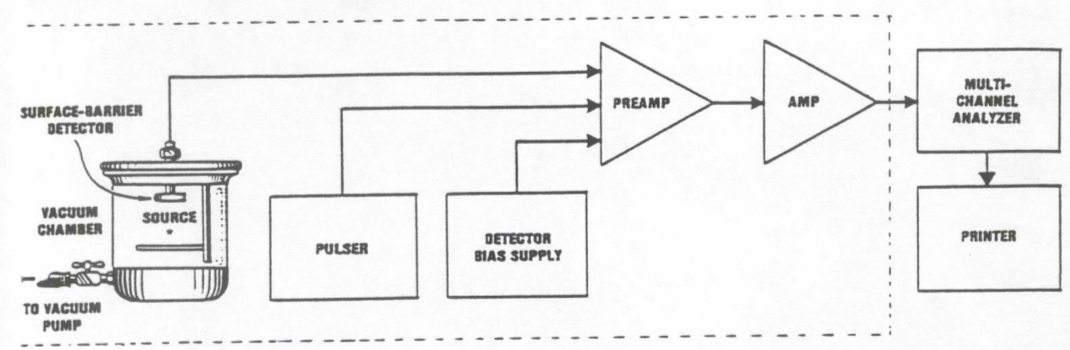
\includegraphics[scale=0.23]{MONT.png}
\caption{Esquema da Montagem}
  \label{fig:sub1}
\end{subfigure}%
\begin{subfigure}{.5\textwidth}
  \centering
  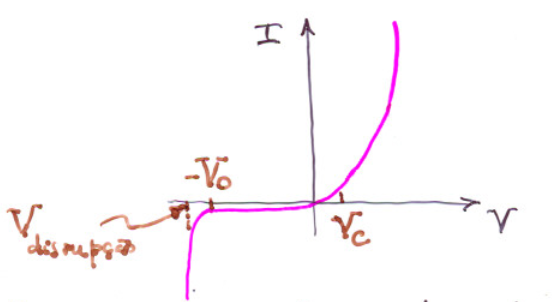
\includegraphics[scale=0.3]{juncpn.png}
\caption{Caraterística Tensão-Corrente de uma junção PN}
  \label{fig:sub2}
\end{subfigure}
\label{fig:test}
\end{figure}

\end{frame}


%%%%%%%%%%%%%%%%%%%%%%%%%%%%%%%%%%%%%%%%%%%%%%%%%%%
\begin{frame}

\frametitle{Espectro de $\ce{^{137}_{55}Cs}$}\framesubtitle{Calibração}

   \centering
   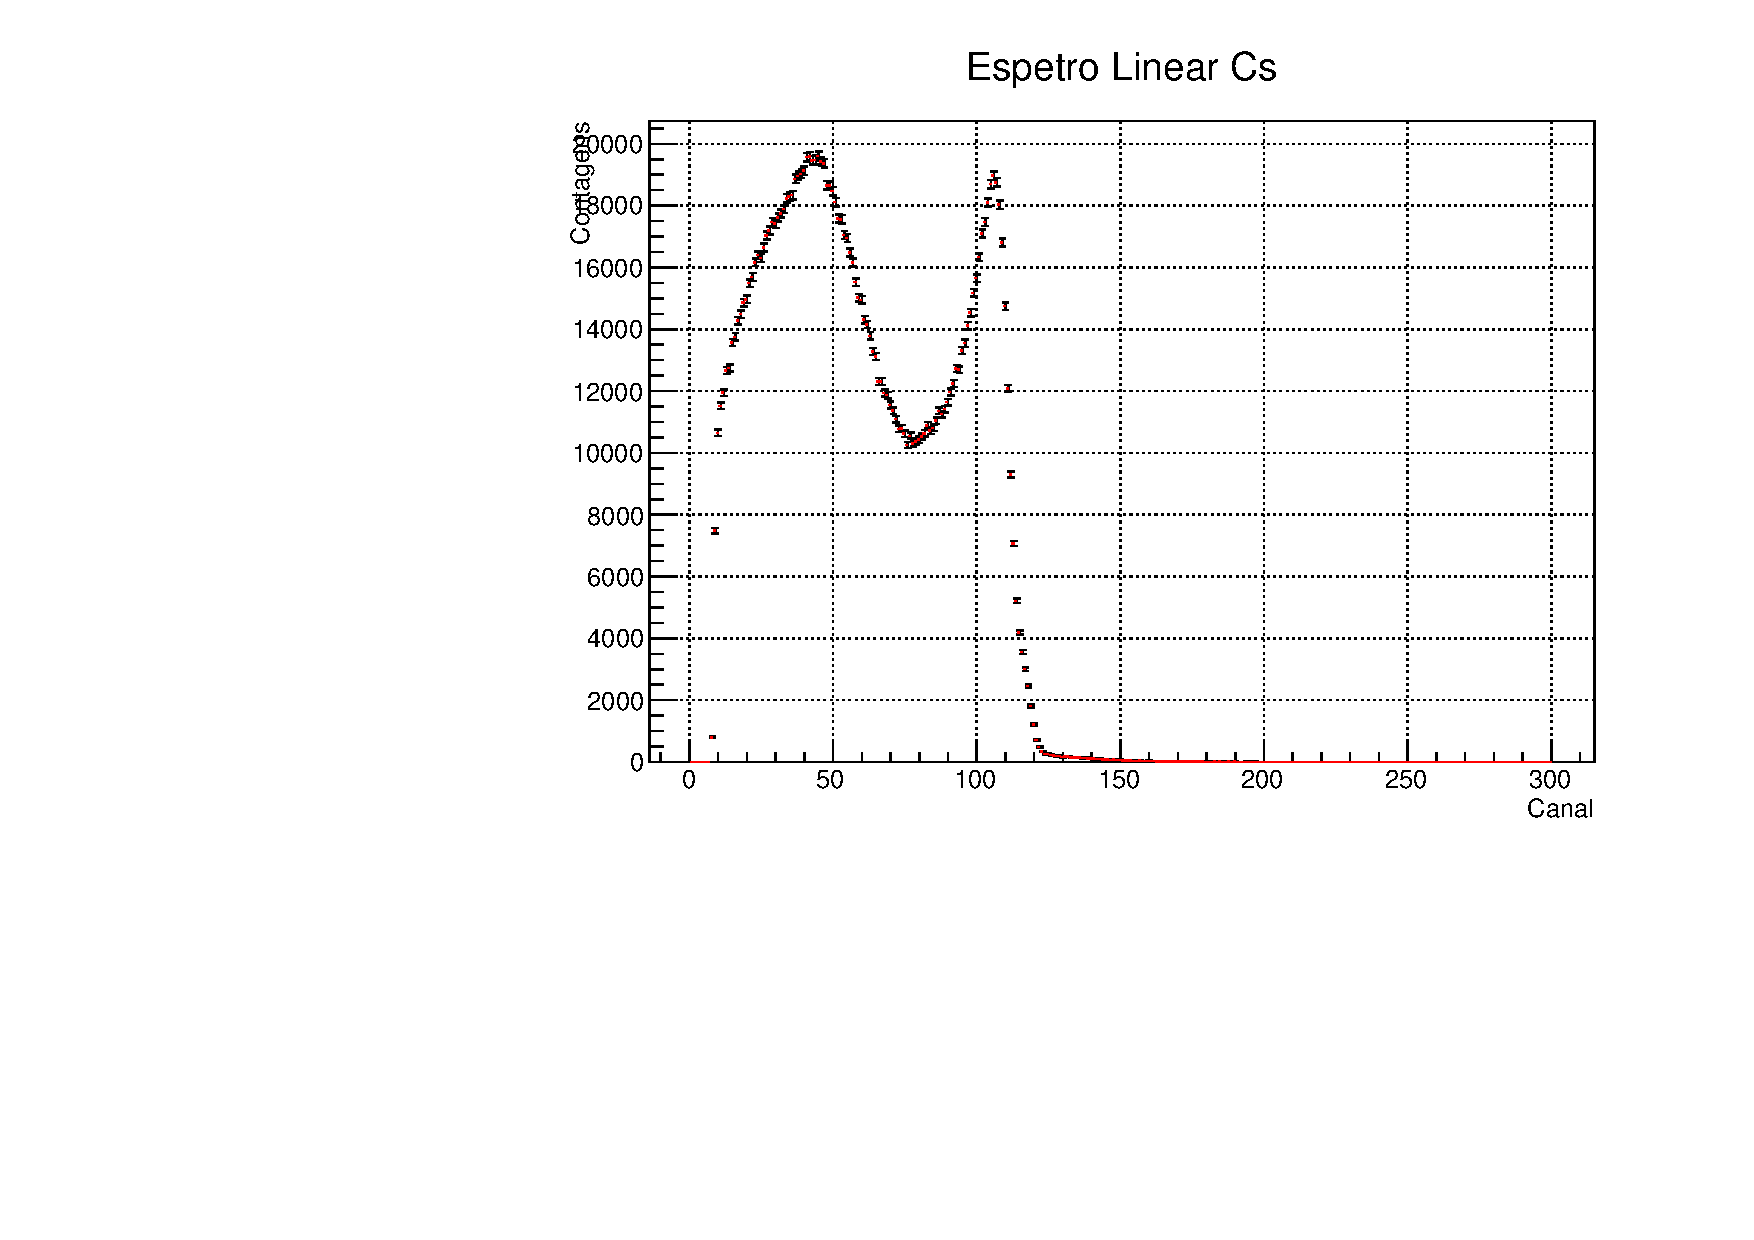
\includegraphics[scale=0.25]{esplincs.pdf}
   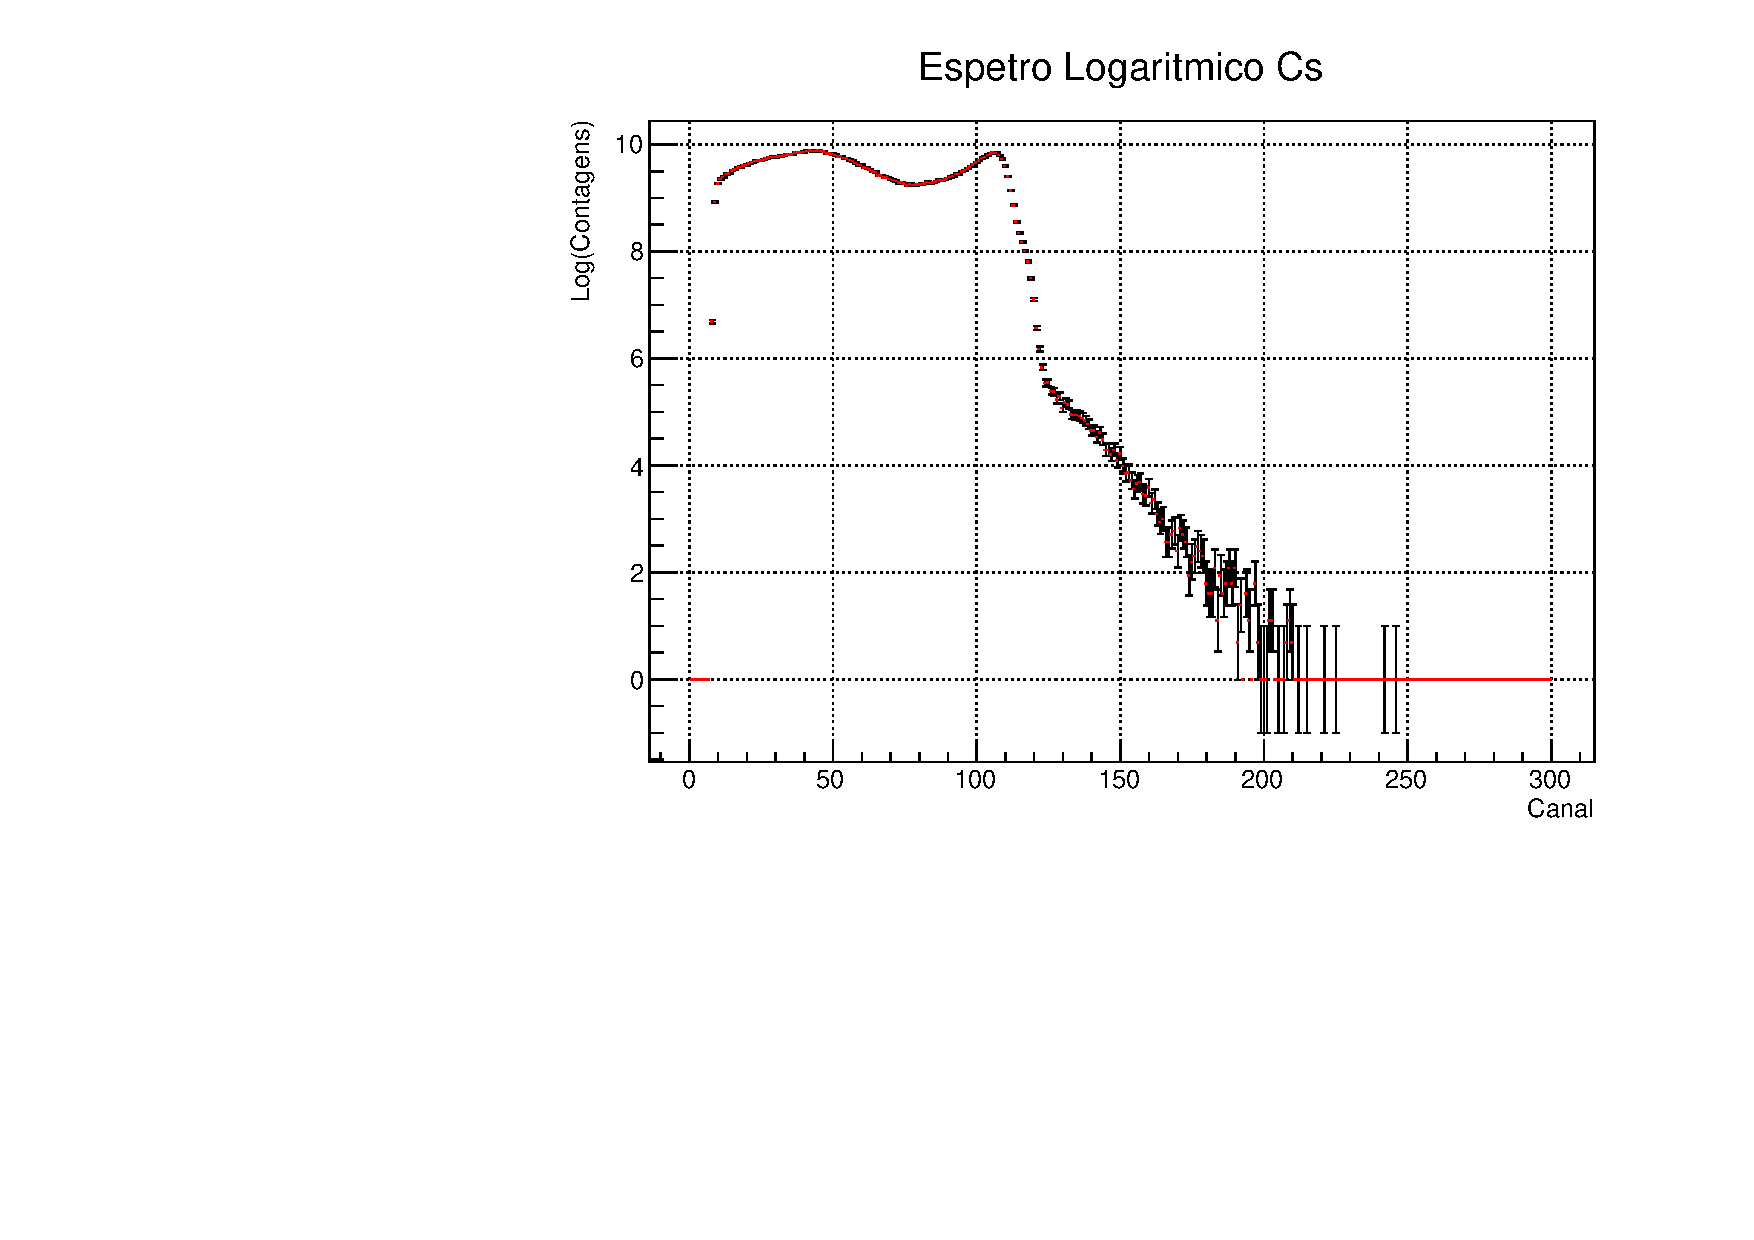
\includegraphics[scale=0.25]{esplogcs.pdf}

\end{frame}


\begin{frame}
\frametitle{Calibração canal-tensão}
\framesubtitle{Calibração}

\begin{equation}
\overline{c}=\frac{\sum\limits_{n=1}^n c_{i}n_{i}}{A}
\label{centroide}
\end{equation}


\begin{equation}
A=\sum\limits_{n=1}^n n_{i}
\end{equation}


\begin{equation}
\sigma_{\overline{c}}=\frac{\sqrt{\sum\limits_{n=1}^n (c_{i}-\overline{c})^2 \cdot n_{i}    }}{A}
\label{e_centroide}
\end{equation}

\end{frame}


\begin{frame}
\frametitle{Calibração canal-tensão}
\framesubtitle{Calibração}
  
\centering
\begin{table}[h]
    \scalebox{0.3}{
        \begin{tabular}{l|llll} 
            \hline
            \hline
             Tensão(V) &    Canal   &     Contagens & Canal Médio & Contagens Totais\\                \hline \hline
                                & \multicolumn{1}{l}{41} & \multicolumn{1}{l}{106} & \\
                                 & \multicolumn{1}{l}{42} & \multicolumn{1}{l}{1028} &\\
                                 & \multicolumn{1}{l}{43} & \multicolumn{1}{l}{1180} &\\
                                0.2 & \multicolumn{1}{l}{44} & \multicolumn{1}{l}{113}&  $ 42.54 \pm 0.01 $& $ 2429 \pm 10 $\\
                                 & \multicolumn{1}{l}{45} & \multicolumn{1}{l}{1}&  \\
                                 & \multicolumn{1}{l}{46} & \multicolumn{1}{l}{1} &\\
                                 \hline  
                                 
                               
                                 
                                  & \multicolumn{1}{l}{85} & \multicolumn{1}{l}{12} & \\
                                 & \multicolumn{1}{l}{86} & \multicolumn{1}{l}{604} &\\
                                  0.4 & \multicolumn{1}{l}{87} & \multicolumn{1}{l}{1477}&  $ 86.88 \pm 0.01 $ & $ 2427 \pm 3 $\\
                                 & \multicolumn{1}{l}{88} & \multicolumn{1}{l}{328} &\\
                               
                                 & \multicolumn{1}{l}{89} & \multicolumn{1}{l}{6}&  \\\hline

                                & \multicolumn{1}{l}{131} & \multicolumn{1}{l}{40} & \\
                                 & \multicolumn{1}{l}{132} & \multicolumn{1}{l}{699} &\\
                                    0.6    & \multicolumn{1}{l}{133} & \multicolumn{1}{l}{1424} & $ 132.79 \pm 0.01 $ & $ 2427 \pm 6 $
 \\ 
                                 & \multicolumn{1}{l}{134} & \multicolumn{1}{l}{260}& \\
                                 & \multicolumn{1}{l}{135} & \multicolumn{1}{l}{4}&  \\\hline
                                 
                                 & \multicolumn{1}{l}{174} & \multicolumn{1}{l}{6} & \\
                                 & \multicolumn{1}{l}{175} & \multicolumn{1}{l}{224} &\\
                                    0.8    & \multicolumn{1}{l}{176} & \multicolumn{1}{l}{1434} & $ 176.23 \pm 0.01 $ & $ 2428 \pm 2 $ \\ 
                                 & \multicolumn{1}{l}{177} & \multicolumn{1}{l}{735}& \\
                                 & \multicolumn{1}{l}{178} & \multicolumn{1}{l}{29}&  \\\hline
                                 
                                & \multicolumn{1}{l}{219} & \multicolumn{1}{l}{2} & \\
                                 & \multicolumn{1}{l}{220} & \multicolumn{1}{l}{229} &\\
                                    1    & \multicolumn{1}{l}{221} & \multicolumn{1}{l}{1368} & $ 221.26 \pm 0.01 $ & $ 2428 \pm 1 $\\

 
                                 & \multicolumn{1}{l}{222} & \multicolumn{1}{l}{791}& \\
                                 & \multicolumn{1}{l}{223} & \multicolumn{1}{l}{38}&  \\\hline
                    
                     & \multicolumn{1}{l}{260} & \multicolumn{1}{l}{33} & \\
                                 & \multicolumn{1}{l}{261} & \multicolumn{1}{l}{95} &\\
                                 & \multicolumn{1}{l}{262} & \multicolumn{1}{l}{1054} &\\
                                1.2 & \multicolumn{1}{l}{263} & \multicolumn{1}{l}{1137}&  $ 262.49 \pm 0.01 $ & $ 2427 \pm 2 $\\
                                 & \multicolumn{1}{l}{264} & \multicolumn{1}{l}{108}&  \\
                                 
                                 \hline  
                                 \hline
        \end{tabular}}
        \end{table}
     
     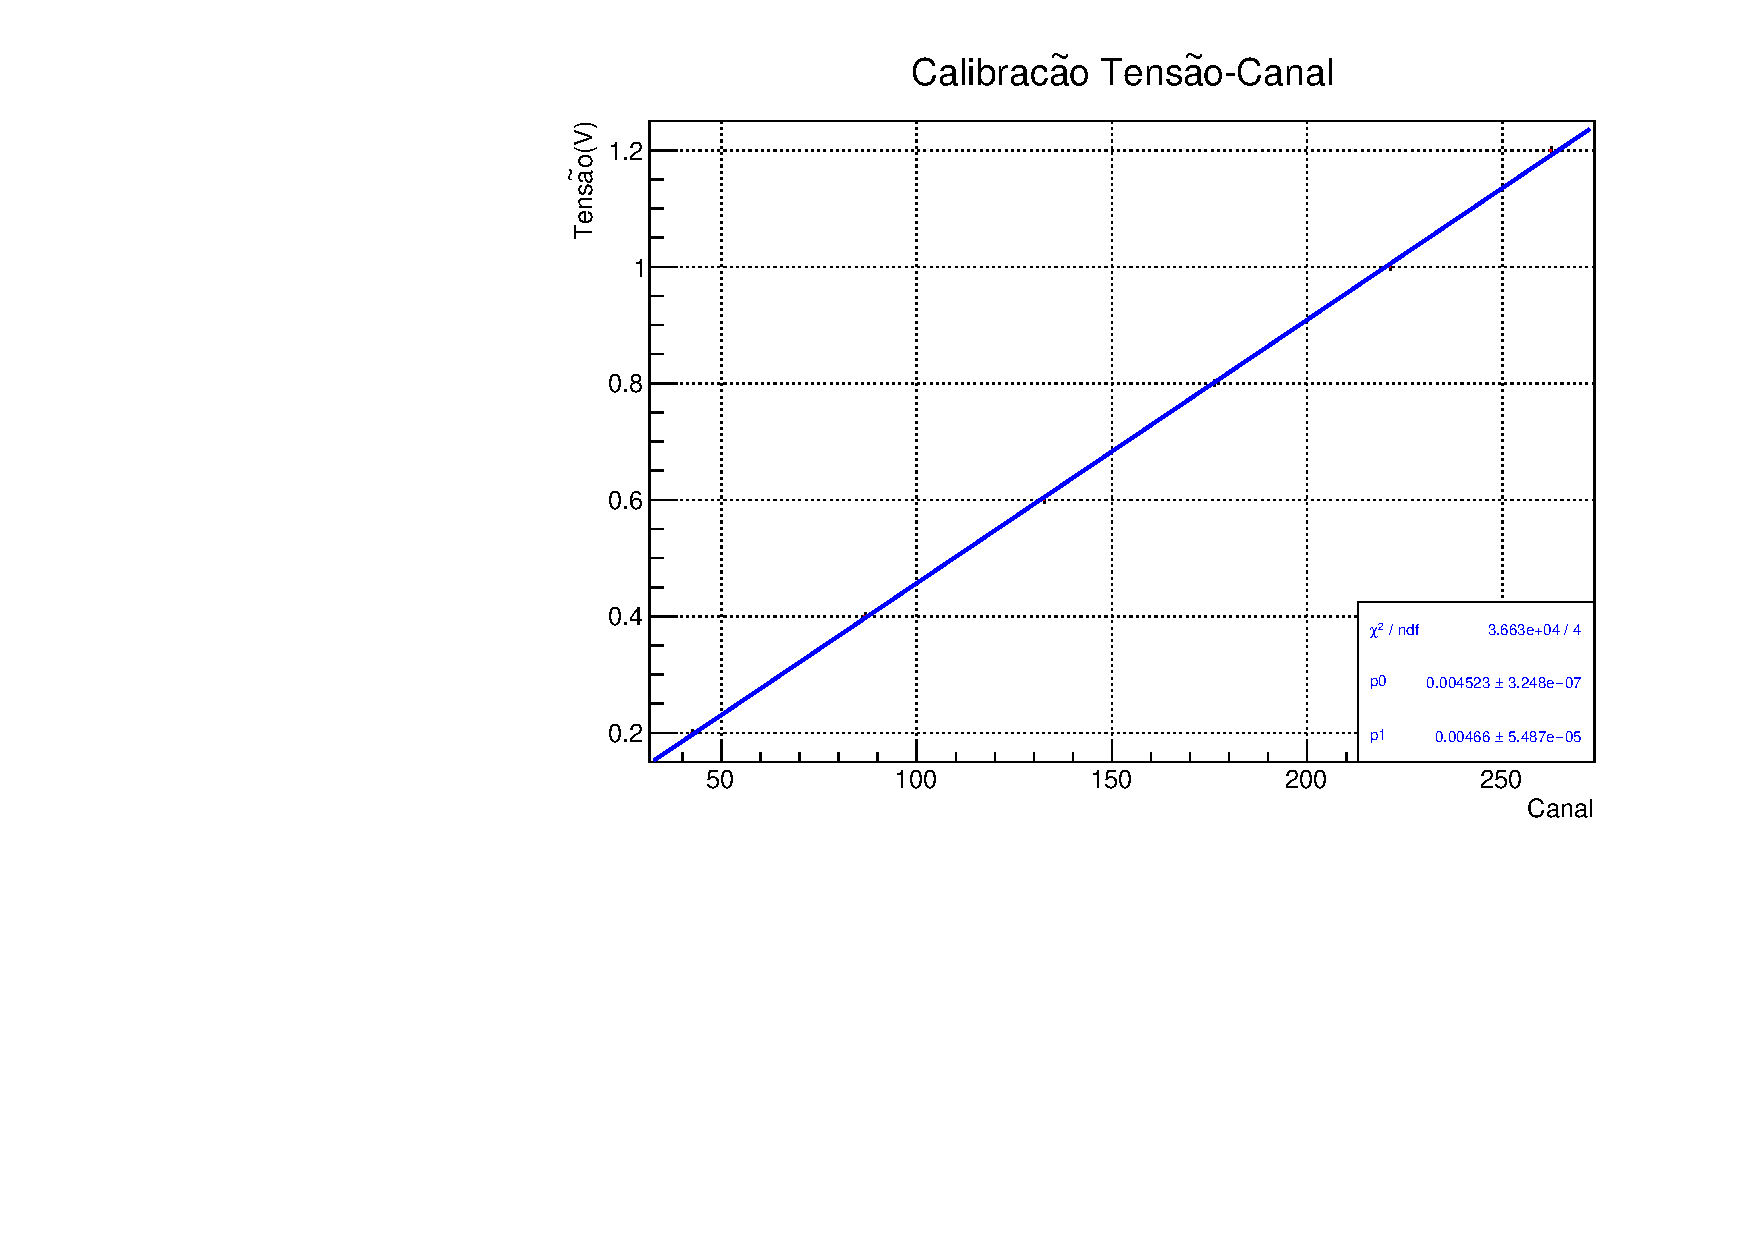
\includegraphics[scale=0.25]{calib2.pdf}

\end{frame}

%%%%%%%%%%%%%%%%%%%%%%%%%%%%%%%%%%%%%%%%%%%%%%%%%%%
%\section{Endpoint de $\ce{^{204}_{81}Tl}$}
\begin{frame}
\frametitle{Espectro de $\ce{^{204}_{81}Tl}$}
\framesubtitle{Endpoint de $\ce{^{204}_{81}Tl}$}

  

\end{frame}

\begin{frame}\frametitle{Ajuste de Kurie}\framesubtitle{Endpoint de $\ce{^{204}_{81}Tl}$}

  

\end{frame}

\begin{frame}\frametitle{Ajuste de Kurie}\framesubtitle{Endpoint de $\ce{^{204}_{81}Tl}$}

 

\end{frame}


\begin{frame}\frametitle{Ajuste de Kurie}\framesubtitle{Endpoint de $\ce{^{204}_{81}Tl}$}


\end{frame}

\begin{frame}\frametitle{Estudo do espectro do $\ce{^{207}_{83}Bi}$}

 
   \centering
   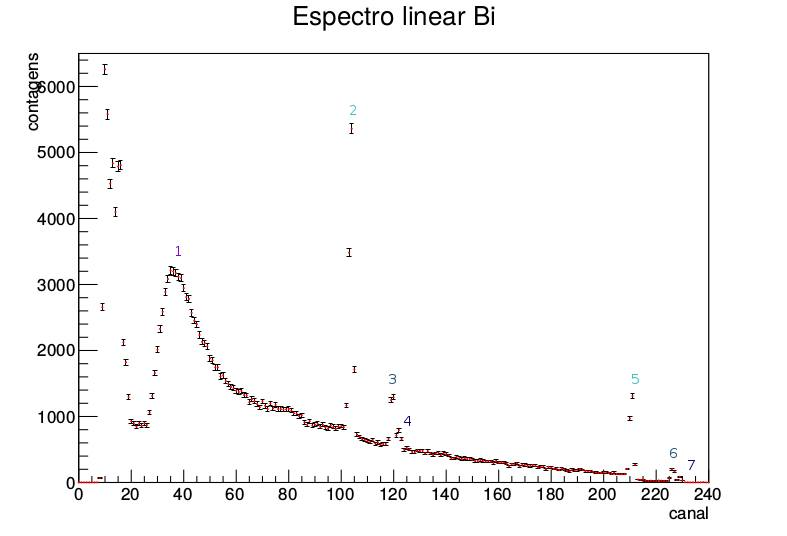
\includegraphics[scale=0.25]{espectro_bi.jpg}
  

\end{frame}

\begin{frame}\frametitle{Regraduação da calibração}

\end{frame}

\begin{frame}\frametitle{Picos de conversão interna}

  

\end{frame}

\begin{frame}\frametitle{Rácios entre áreas dos picos de conversão interna}

 

\end{frame}














\begin{frame}\frametitle{Ajuste de Kurie}%\framesubtitle{Endpoint de $\ce{^{204}_{81}Tl}$}
\centering

\begin{figure}

\begin{subfigure}

 \begin{tabular}{c|c}
  \hline \hline
  Parâmetros & Valor \\
  \hline
  \hline
  E0 ($keV$)     & $713.66 \pm  4.82 $\\
  K ($MeV^{-1}$) & $5.90   \pm  0.12 $\\
  $\chi^2/\nu$   & 2.26 \\ \hline \hline
 \end{tabular}
%\caption{Parâmetros do ajuste do plot de Kurie}
%\label{tabKurie}
\end{subfigure}

\begin{subfigure}
 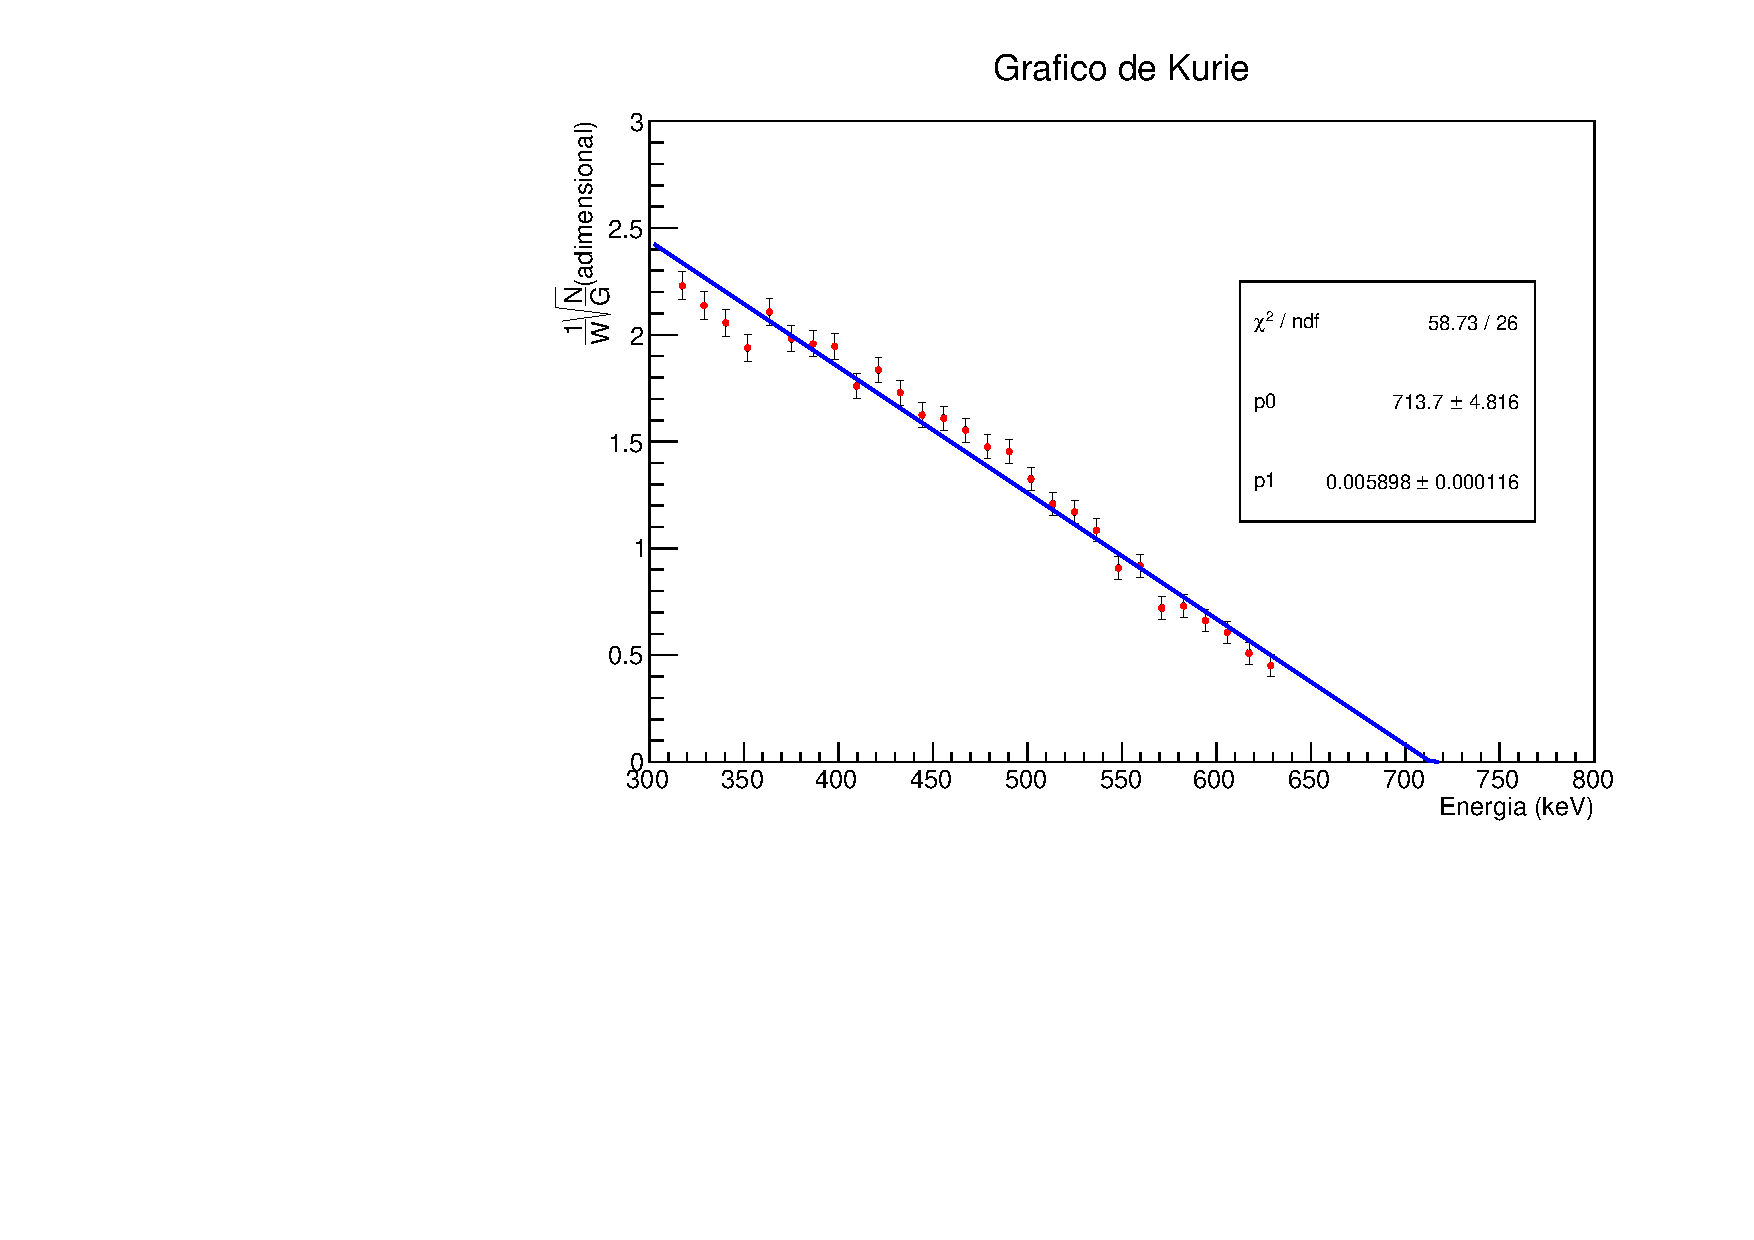
\includegraphics[scale=0.45]{Kurie.pdf}
\end{subfigure}

\end{figure}



\end{frame}

\end{document}
